\chapter{Stand des Wissens und der Technik}
\section{Funktionsweise eines Prozessor}

Ein Prozessor ist eine universelle Rechnermaschine, die sich durch eine definierte Reihe von Anweisungen programmieren lässt. Zu den arithmetische Anweisungen gehört der Zugriff auf Speicheradressen und Sprünge innerhalb der Abfolge der Anweisungen.
Bereits der britische Mathematiker Alan Turing konnte aufzeigen, dass ein universelles Berechnungsmodell möglich ist wenn ein Rechner neben Speicherzugriff auch Sprünge besitzt\cite{Hoffmann2014l}. Auf diese besondere Eigenschaft sind die heutigen Prozessoren aufgebaut. Ein Programm das der Prozessor ansteuert, besteht aus einer endliche Anzahl von geordnete Anweisungen. Der Prozessor befolgt, streng nach dem Ablauf Anweisungen für Anweisung, die auch Sprünge zu einer andere Stelle innerhalb des Programm besitzen.
\par
Die Prozessoren, auch Zentraleinheit oder CPU genannt, besitzen im inneren drei Einheiten die über ein Datenbus verbunden sind. Dies ist in \autoref{fig:CPU} ersichtlich. Dabei kann der Datenbus je nach Grösse oder Leistung des CPU variieren. Die meist verbreiteten CPU, die in den heutigen PC verbaut sind haben ein 64bit-Datenbus. In dieser Arbeit werden aber mit kleinere CPUs gearbeitet die einen 32bit-Datenbus besitzen. Die Control Unit\cite{patterson2013computer} ist verantwortlich, dass das Programm immer an der richtige Stelle ausgeführt wird. Sie nimmt Anweisungen an, dekodiert sie und übergibt sie der ALU. Die Übergabe erfolgt durch die Weichenstellung des Datenbus der ALU und Register. Die Arithmetic and Logical Unit ermöglicht es Rechenoperationen sowie logische Operationen an den Daten auszuführen. Die Register haben die Grösse des Datenbus und dienen dazu, die Daten von und zur ALU zu bewegen. Ein CPUs besitzt mehrere Register und variiert je nach CPU-Architektur. Die Register lassen sich in zwei Kategorien, Universal- und Hilfsregister unterteilen. In den Universalregister lassen sich die zu bearbeitende Daten speichern. Die Hilfsregister haben eine besondere Rolle zugeordnet. Als Beispiel zählt der Statusregister zum Hilfsregister, der Aufschluss gibt über das Resultat der vorherige Operation. So lässt es sich über diesen Hilfsregister herauslesen ob eine Operation von zwei Zahlen zum Überlauf gekommen ist.
Da die Anzahl meist sehr klein ist, müssen die Daten immer wieder, von den Register in den RAM und wieder zurück geladen werden.
\par
Prozessoren sind als elektronische Schaltkreise realisiert und werden durch die Halbleiter Technologie hergestellt. Die Millionen von witzigen Transistoren die ein Prozessor beinhaltet werden zu logische Bausteine verdrahtet.
\par
In dieser Arbeit ist die Funktionsweise der ALU relevant. Wir wissen, dass die ALU eine Reihe von Anweisungen erhält und somit jeden erdenkbaren Algorithmus ausführen kann. Im Rahmen dieser Arbeit, wird eine Methode Entwickelt, damit der Energie verbrauch einer Einzelne Anweisung der ALU Messen können.



\begin{figure}[t]
\centering
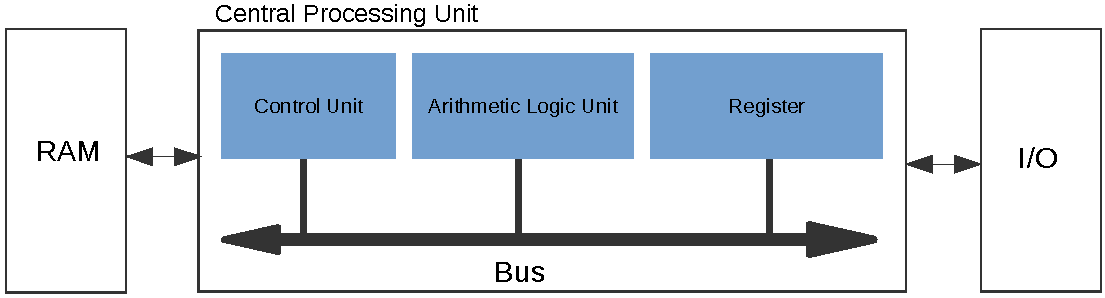
\includegraphics[width=1.0\textwidth]{images/cpu.pdf}
\caption{Central Processing Unit}
\label{fig:CPU}
\end{figure}

\section{Aufbau des Linux Betriebssystem}


\section{Unterschiede CISC und RISC CPUs}



\section{Energy Storage in a Capacitor}


